\documentclass{article}

\usepackage{graphicx} % Required for the inclusion of images
\usepackage{natbib} % Required to change bibliography style to APA
\usepackage{amsmath} % Required for some math elements 
\usepackage{listings}
\usepackage{mathtools}
\usepackage{float}
\usepackage{authblk}
\usepackage{color}
\usepackage{braket}
\usepackage{url}
\usepackage{hyperref}
%\usepackage{verbetim}
%\usepackage{physics}
%\usepackage{siunitx}

\urlstyle{rm} % Roman font family for URL's

\usepackage[T1]{fontenc}
\usepackage{verbatimbox}

\usepackage[margin=1in]{geometry} % Margin Size

\setlength\parindent{0pt} % Removes all indentation from paragraphs

\usepackage{times} % Use the Times New Roman font

%----------------------------------------------------------------------------------------
%	DOCUMENT INFORMATION
%----------------------------------------------------------------------------------------

\begin{document}
\section{Computing Weights from ten Digitized Samples} 

\subsection{Computational Method} 



\subsection{Megan's Branch:}
\subsubsection{Where to Find Needed Files and Directories} 
This branch of the directory can be found at the following link:
\href{https://github.com/atishelmanch/ECAL_Weights/tree/Megan}{\bf{Megan's Branch}}\\
\begin{comment}
Overview of Repository Branch: 
\\Data: All input data needed
\\sourcecode: CLHEP, standard directories, etc. 
\\src: ComputeWeights is the branch that this manual focusses on
\\ src/ComputeWeights: 
\begin{itemize} 
\item \begin{verbatim} Calculate.cpp \end{verbatim}
\item \begin{verbatim} CalculateWeights.py \end{verbatim}
\item  \begin{verbatim} ComputeWeights.cpp \end{verbatim}
\item \begin{verbatim} ComputeWeights.h \end{verbatim}
\item \begin{verbatim} Calculate_AlphaBeta.cpp \end{verbatim}
\item \begin{verbatim} Untitled.cpp \end{verbatim}
\item \begin{verbatim} Plot_AlphaBetaWeights.py \end{verbatim}
\item \begin{verbatim} alphabeta_rootcode.cpp \end{verbatim}
\end{itemize}
\end{comment}

%$$ https://github.com/atishelmanch/ECAL_Weights/tree/Megan $$ 
%This directory is located at the following link:
%\href{https://github.com/atishelmanch/ECAL_Weights/tree/Megan/src/ComputeWeights}{\bf{Compute Weights}}
%$$  https://github.com/atishelmanch/ECAL_Weights/tree/master/src/ComputeWeights $$ 

Details on all files contained in this directory can be found below.

\subsubsection{Determining Weights for 10 digitized samples :Calculate.cpp}

This is a file for extracting weights for reconstruction of pulse shape from 10 digitized data points. %what are these data points of? describe this more? 

\vspace{5mm}

The script reads a text file with 14 tab delineated data points and used the user specified points to calculate corresponding weights accordingly. 
Other files required to run this code are ComputeWeights.cpp and  ComputeWeights.h which can all be found in the following directory:
\href{https://github.com/atishelmanch/ECAL_Weights/tree/Megan/src/ComputeWeights}{\bf{Compute Weights}}

\vspace{5mm}

In addition to those files the machine used will also need the CLHEP directory installed. If the CLHEP directory is needed, use the following link for documentation and installation help: 
\href{http://proj-clhep.web.cern.ch/proj-clhep}{\bf{CLHEP Documentation}}
%$$  http://proj-clhep.web.cern.ch/proj-clhep/ $$ 

% Do we need this? 
% $$ECAL_Weights/sourcecode/bin/ $$ 

\vspace{5mm}

Within the file 'calculate.cpp' the user is able to define the data file they wish to use. This can be done by the user being prompted for the file name inside the terminal or by hardcoding the path of the data file into the script. Data files are currently located in the following directory: 
\href{https://github.com/atishelmanch/ECAL_Weights/tree/Megan/Data}{\bf{Data Files}}. 
\\Original data can also be found at: \href{https://github.com/atishelmanch/ECAL_Weights/tree/Megan/Data}{\bf{Data Files on lxplus}} but access to lxplus is required. %add link andrea originally sent us here in one of his original emails 


\begin{comment}
     \begin{verbatim}
  //user prompt for file name
  cout << "Enter File Name: ";  
  std::string file = "/Users/meganstark/Computation*/PHYS7321_Project/Data/
  template_histograms_ECAL_Run2017_runs_305814_305814.txt" ;

  Comment this out for no file input and will run file listed above
  /*
  std::string input;
  std::cin >> input;
  cin.ignore(100, '\n');
  getline(cin, input);
  if ( !input.empty() ) {
      std::istringstream istr( input );
      istr >> file;
  }
  */
  Stop commenting out here
     \end{verbatim} 
     
Each data file contains $\approx 75k$ lines. The user can specify if they would like to run the entire data file or only a given number of lines in the following code: 

     \begin{verbatim}
  int count = 0;
  while(std::getline(inFile, line)) {
    count = count +1;
    //cout << count << endl;
    if (count == 10) {
      // if want whole file checkvariable set to < 0 
      // i.e. if want 10 lines read set line 79 to "if(count == 10){"
      break;
    } 
     \end{verbatim} 
     

%------------------------------------------------------------------------------------------------------------------------------------------------

Current data file has 14 tab delineated data points, but we currently only take the first 10 samples. The other 4 data points are ....why dont we take the other points ,etc 

     \begin{verbatim} 
     \\ComputeWeights(verbosity, doFitBaseline, doFitTime, nPulseSamples, nPrePulseSamples)
 ComputeWeights A(verbosity, false, true, nSamples,3);
     \end{verbatim} 
       
The file and computes the derivative of the pulse shape using the following method. Explain other calculated 

The function 'function name/ used taking the following variables: 

Verbostiy (Can be set to 0 or 1) : \\ For verbosity set to zero:
   \begin{verbatim} 
   cout << "A.getAmpWeight(i) returns: " << A.getAmpWeight(i) << endl;
For verbosity set to one:
      \end{verbatim}
      
   \begin{verbatim} 
   if (verbosity > 0) {
        cout << "verbosity_ = " << A.GetVerbosity() << endl;
        cout << "doFitBaseline_ = " << A.GetDoFitBaseline() << endl;
        cout << "doFitTime_ = " << A.GetDoFitTime() << endl;
        cout << "nPulseSamples_ = " << A.GetnPulseSamples() << endl;
        cout << "nPrePulseSamples_ = " << A.GetnPrePulseSamples() << endl;

        cout << "A.getAmpWeight(5) returns: " << A.getAmpWeight(5) << endl;
        cout << "A.getChi2Matrix(5,5) returns: " << A.getChi2Matrix(5,5) << endl;
        for(int i = 0; i < pulseShape.size() ; i ++){
          cout << "A.getAmpWeight(i) returns: " << A.getAmpWeight(i) << endl;
          cout << "A.getTimeWeight(i) returns: " << A.getAmpWeight(i) << endl;
        }
      }
      \end{verbatim}

doFitBaseline (Boolean):  If this variable is set to true.......

doFitTime (Boolean): If this variable is set to true weights will be computed taking into account possible time jitter.  

      explain time jitter and why this is needed 
      Same code as compute.cpp with the addition of time jitter simulation 
      
nPulseSamples:  number of samples from which you are reconstructing the pulse shape, usually 10 but can be defined by user
nPrePulseSamples: Number of baseline samples also called the pedestal. 


     \begin{verbatim}
     pulseShapeDerivative[i] =  (pulseShape[i-1] - pulseShape[i]);      
     \end{verbatim} 

And then computes the weights using the following function: 
        \begin{verbatim}
        A.compute(pulseShape,pulseShapeDerivative,tMax); 
         \end{verbatim}

pulseShape: vector of nsamples 
pulseShapederivative: vector of derivative of n samples setting the first derivative equal to 1
tMax:  index  of the maximum value of nsamples       

explanation of calculation 
Running this file prints out the following variables in the terminal:

\indent For verbosity set to zero:

   \begin{verbatim} 
   cout << "A.getAmpWeight(i) returns: " << A.getAmpWeight(i) << endl;
\indent For verbosity set to one:
      \end{verbatim}
   \begin{verbatim} 
   if (verbosity > 0) {
        cout << "verbosity_ = " << A.GetVerbosity() << endl;
        cout << "doFitBaseline_ = " << A.GetDoFitBaseline() << endl;
        cout << "doFitTime_ = " << A.GetDoFitTime() << endl;
        cout << "nPulseSamples_ = " << A.GetnPulseSamples() << endl;
        cout << "nPrePulseSamples_ = " << A.GetnPrePulseSamples() << endl;

        cout << "A.getAmpWeight(5) returns: " << A.getAmpWeight(5) << endl;
        cout << "A.getChi2Matrix(5,5) returns: " << A.getChi2Matrix(5,5) << endl;
        for(int i = 0; i < pulseShape.size() ; i ++){
          cout << "A.getAmpWeight(i) returns: " << A.getAmpWeight(i) << endl;
          cout << "A.getTimeWeight(i) returns: " << A.getAmpWeight(i) << endl;
        }
      }
      \end{verbatim}


The script then saves the pulse shape data and corresponding weights to a tab delineated output file of the following format:

      %saving pulseshape and the weights to output file
      %file format:
      \begin{verbatim}    //[pulsenumber samplept1 samplept2 samplept3 ......samplept10 weightpt1 weightpt2 ...... weightpt10]
      output_file << d2 << "\t"; //       
      \end{verbatim}

saving pulse number to output file
 \end{comment}
%------------------------------------------------------------------------------------------------------------------------------------------------
\subsubsection{Running the File in Terminal}   
   
To run these files in terminal run the following command: %need to make it a more generic command

\begin{verbatim} 
 clang++ -std=c++11 -stdlib=libc++ -L/Users/meganstark/Computation\*/
 PHYS7321_Project/sourcecode/bin/lib/ -I/Users/meganstark/Computation
 \*/PHYS7321_Project/sourcecode/bin/ -lCLHEP-Matrix-2.3.4.5  
 Calculate.cpp ComputeWeights.cpp      
\end{verbatim}

Below is an example: 

\begin{verbatim} 
 clang++ -std=c++11 -stdlib=libc++ -L/Users/meganstark/Computation\*/
 PHYS7321_Project/sourcecode/bin/lib/ -I/Users/meganstark/Computation
 \*/PHYS7321_Project/sourcecode/bin/ -lCLHEP-Matrix-2.3.4.5  
 Calculate.cpp ComputeWeights.cpp      
\end{verbatim}
      
      
      This command will create an output file called 'a.out' in the current directory. To run this file use the following command in the terminal:
      
 \begin{verbatim}    
./a.out 
\end{verbatim}
      
     
      then run this file and saves output file that includes weights also depending on the set verbosity will output the variables noted above in the terminal. The output file is currently saving files to the following directory: 
      
      and is of the following format: 
\begin{comment}
\subsubsection{Brief Aside on Other Files need to run the above commands and Scripts} 

ComputeWeights.cpp and  ComputeWeights.h
CLHEP 
Root
std directory 

\end{comment}

     %\subsection{ComputeWeights.cpp}
     %\subsection{ComputeWegihts.h}
          \subsubsection{TimeWeights.py}     
          
          This script plots the output data of Calculate.cpp. 
     \subsubsection{CalculateWeights.py}
     
This file is a less robust version of the same calculation in python. It is convenient however, since a single script is able to run make the calculations as well as plot the results. 


%% -----------------------------------------------------------------------------------------------------------------------------------

\section{Computing Weights From Alpha and Beta Parameters} 

\subsection{Determining Ten Samples from the Pulse} 

\subsubsection{Determining Ten Samples in Root Terminal} 
User will need to input the following variables: alpha, beta, t0, amplitude 
\\ Values for these variables can be found below. \\
$ /Users/meganstark/Computation*/PHYS7321_Project/Data/CrystalParams.txt $ \\ %need to change this path to git 
This file containes these four variables for each of the $\approx 75k$ crystals in the ECAL. 
\\

	
The format of the file is shown below: 
		\begin{verbatim} 
					Crystal ID#  Amplitude T0     Alpha    Beta 
			838861313    0.240791  121.44 1.18942  40.1906
\end{verbatim}

User will also need to input the number if iterations $i$ which is the number of time shifted samples that will be determined. Each time the code iterates over $i$, the sample is taken from original sample location + 1 x-unit. For example, the 10th iteration will be taken from original sample location + 10. 

\vspace{2mm}
To use the Fit Alpha Beta function in order to determine the 10 samples for a given alpha beta value can be done using the following commands in the terminal. 
\vspace{2mm}
In order to do this you must have ROOT installed on your computer. If ROOT has not been installed documentation on ROOT can be found here: \href{https://root.cern.ch}{\bf{ROOT Documentation}}.

I used HomeBrew to install ROOT on my Mac OS. Homebrew can be found here: \href{https://brew.sh}{\bf{HomeBrew}}.

\vspace{2mm}

To open ROOT use the following command in the terminal:

\begin{verbatim} 
root -l  //open root 
\end{verbatim}

Then the function needs to be defined, here TF1 is a predefined data type in ROOT. When defining the function the final two imput variables must be changed. These are the minimum and maximum variables on the x axis. 
\begin{verbatim} 
TF1 *function_alphabeta = new TF1("function_alphabeta","[0] * 
pow(1 + (x-[1]) / ([2]*[3]) , [2] ) * exp ( - (x-[1]) / [3])",73,40*10.5);
// definition of the alpha beta function: 
// TF1("function name" , function definition, xmin, xmax);
// Here, [0], [1], [2], and [3] are the needed parameters;
  \end{verbatim}
  
Next, the user need to set the parameters as mentioned above. These parameters should be from a single crystal (single line) from crystalparams.txt and set the following parameters with the following code, where within the parentheses is the parameter number, and then the parameter value. Parameter $0$ is the amplitude, parameter $1$ is $t_0$, parameter $2$ is Alpha, and parameter $3$ is Beta. 

 \begin{verbatim} 
function_alphabeta->SetParameter (0, 0.240791);    // A 
function_alphabeta->SetParameter (1, 121.44);   // t_0 
function_alphabeta->SetParameter (2, 1.18942);   // alpha 
function_alphabeta->SetParameter (3, 40.1906);   // beta 
\end{verbatim}

In order to see the pulse one should use the following command: 
 \begin{verbatim} 
function_alphabeta->Draw()
\end{verbatim}

If one is not able to see the pulse in its entirety (see image before for example) The one must change the range on the x axis. To do this you should use the following command: 

 \begin{figure}[h!] 
    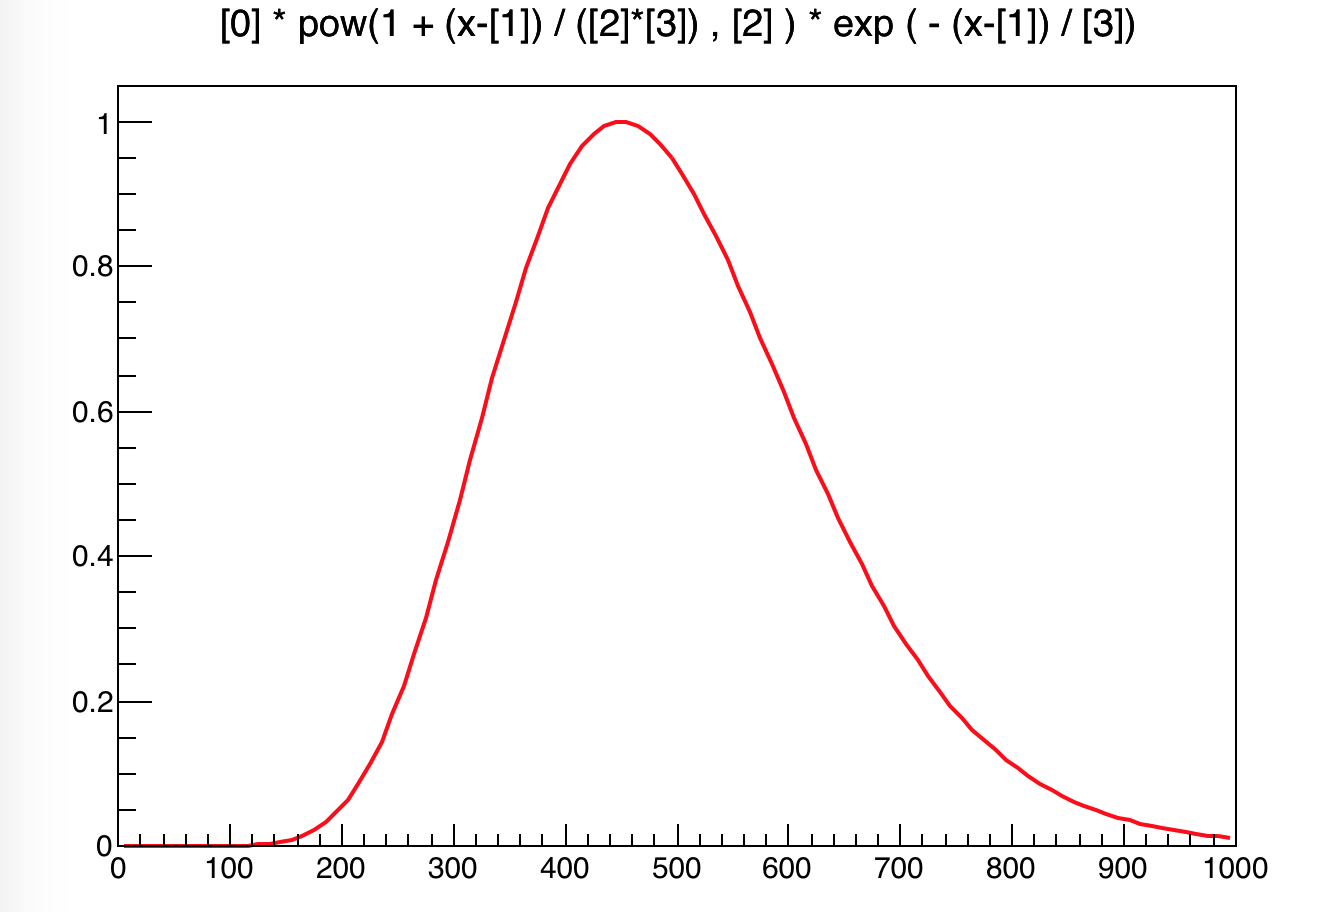
\includegraphics[width=.5\linewidth]{pulse2.png} 
 \end{figure} 
 
 \begin{verbatim} 
function_alphabeta->SetRange(71, 400) // setting range of x axis in the 
// entire pulse is not able to be seen 
function_alphabeta->Draw() // Make sure to draw the function again 
// to know for sure you have the proper xmin and x max 
\end{verbatim}

You will then want to redraw the pulse and continue to follow this process until the entire pulse can be seen in the plot. 
\\
\vspace{5mm}

Next we will want to create an output file for the 10 samples being extracted will be saved to. This is done using the following command: 

\begin{verbatim} 
  std::chrono::system_clock::time_point tp = std::chrono::system_clock::now();
  std::chrono::system_clock::duration dtn = tp.time_since_epoch();
  std::stringstream ss;
  ss << "output/" << "new17" << ".txt";
  std::ofstream output_file(ss.str());
  // creating output folder for the sample results to be saved to 
\end{verbatim}




%%
% add comments for the below section 
%how to best explain?
\begin{verbatim} 
std::vector<double> d;
\end{verbatim}
// determining samples for i iterations 
//each iteration the sample is taken from the ith unit to the left. This is for the calculation of time shifting . 

\begin{verbatim} 
for(int i = 1;i<20;i++){
    for(int j = 0;j<90*9+i;){
        double tmp = function_alphabeta->Eval(i + j);
        d.push_back(tmp);       
        j = j + 90;
    }
}

\end{verbatim}
//saving to tab delineated output file with name given above 

\begin{verbatim} 
for(int k = 0; k<d.size(); k++){ 
    int lineLength = k % 10; 
    if(lineLength < 9){  
        output_file << d[k] << "\t";
    } else {
        output_file << d[k] << "\n";     
    }
}
\end{verbatim}
%%




From these commands a single file will be created with 10 samples saved for each iteration over $i$ (moving one x units to the left). \\ This file will be saved to the following directory: $/Users/meganstark/Computation*/PHYS7321_Project/output/$ %change to git dir. 
\\ The file will be given the name titled above, here it is$ "new17.txt"$ User should change the file name. \\
\\ The saved file will have the following format:
\begin{verbatim} 
for i = 0:  sample1 sample 2 sample 3...
\end{verbatim}
Each line in the file should contain $10$ tab delineated values, there are the$ 10$ samples from that pulse.
This file can then be used as an input for the method mentioned above in order to determine the weights for the $10$ samples. See section 2.2 for more details. %add section number for reference  




%-------------------------------------------------------------------------------------------------------------------------------------------
\subsubsection{Script to Determine 10 Samples: Untitled.cpp} 

$Untitled.cpp$ reads a text file with tab delineated crystal parameters, and uses the user specified points to calculate corresponding samples of the created pulse. 
Other files required to run this code are:
\\
 which can all be found in the following directory:
\href{https://github.com/atishelmanch/ECAL_Weights/tree/Megan/src/ComputeWeights}{\bf{Compute Weights}}
\\
% add git path for file 

User defined input variables for the script: $xmin$ , $xmax$, number of iterations $i$ , and the file CrystalParams.txt located in the following directory:
	\begin{verbatim} /Users/meganstark/Computation*/PHYS7321_Project/Data/CrystalParams.txt \end{verbatim} 
		format of file: 
		\begin{verbatim} 
					Crystal ID#  Amplitude T0 		     Alpha    Beta 
	838861313    0.240791  121.44   1.18942  40.1906
		\end{verbatim}

To build this file use the following command:

\begin{verbatim} 
clang++ -std=c++11 -stdlib=libc++ -v `root-config --cflags --glibs --libs` 
-L/Users/meganstark/Computation\*/PHYS7321_Project/sourcecode/bin/lib/ -I/Users
/meganstark/Computation\*/PHYS7321_Project/sourcecode/bin/root/hist/hist/inc/ 
-I/Users/meganstark/Computation\*/PHYS7321_Project/sourcecode/bin/root/include/ 
-I/Users/meganstark/Computation\*/PHYS7321_Project/sourcecode/bin/root 
-lCLHEP-Matrix-2.3.4.5 /Users/meganstark/Computation\*/PHYS7321_Project/src/
ComputeWeights/untitled.cpp -o /Users/meganstark/Computation\*/PHYS7321_Project/a.out
\end{verbatim}

% describe this command in detail and change paths to git paths? 

The executable file will be located in: \begin{verbatim} PHYS7321_Project/\end{verbatim}   %change to git dir. 
and will be named \begin{verbatim} a.out \end{verbatim}. 

The following command can then be used to execute the file: 
 \begin{verbatim} ./a.out  \end{verbatim} 

Executing this file will will create an output file in the following directory: 
$Users/meganstark/Computation*/PHYS7321_Project/output/$ %change to git dir. 
\\ The saved file will have the following format:
\begin{verbatim} 
for i = 0:  sample1 sample 2 sample 3...
\end{verbatim}
Each line in the file should contain $10$ tab delineated values, there are the$ 10$ samples from that pulse.
This file can then be used as an input for the method mentioned above in order to determine the weights for the $10$ samples. See section 2.2 for more details. %add section number for reference  

%-----------------------------------------------------------------------------------------------------------------------------
\subsection{Determining Weights From Alpha Beta Parameters: $Calculate_{}AlphaBeta.cpp$}

$Calculate_{}AlphaBeta.cpp$ reads a text file with 10 tab delineated data points and uses the user specified points to calculate corresponding weights accordingly. 
Other files required to run this code are ComputeWeights.cpp and  ComputeWeights.h which can all be found in the following directory:
\href{https://github.com/atishelmanch/ECAL_Weights/tree/Megan/src/ComputeWeights}{\bf{Compute Weights}}


input: file of data samples determined using Untitled.cpp or the Code noted above for the root terminal 

running: 
following code to build: 

\begin{verbatim} 
clang++ -std=c++11 -stdlib=libc++ -L/Users/meganstark/Computation*/PHYS7321_Project/
sourcecode/bin/lib/ -I/Users/meganstark/Computation*/PHYS7321_Project/sourcecode/bin/ 
-lCLHEP-Matrix-2.3.4.5 /Users/meganstark/Computation*/PHYS7321_Project/src/
ComputeWeights/Calculate_AlphaBeta.cpp /Users/meganstark/Computation*
/PHYS7321_Project/src/ComputeWeights/ComputeWeights.cpp -o /Users/meganstark/
Computation*/PHYS7321_Project/a.out
\end{verbatim}

will give an executable a.out in following directory: 

this output will have the following form: 

Execute this file using following command: ./a.out 

In turn, this will give you an output file of the following name with the following format 

%------------------------------------------------------------------------------------------------------------------------------------------------
\subsection{Plotting Results:  $ Plot_{}AlphaBetaWeights.py  $ } 

Input variables: 

User will need to input the file with weights, located on line 27 :
\begin{verbatim} 
with open('new18_weights.txt', 'r') as f:  
\end{verbatim}
Here it is opening \begin{verbatim}  new18_{}weights.txt \end{verbatim}.

This file will plot the samples, weights, and amplitude of signal located in the input file. 

%------------------------------------------------------------------------------------------------------------------------------------------------
\begin{comment}
\subsection{Current Results} 

Add plots from last powerpoint presentation 
\end{comment}

%------------------------------------------------------------------------------------------------------------------------------------------------
\section{References} 

\begin{itemize}

\item \href{http://cds.cern.ch/record/933702?ln=en}{\bf{Reconstruction of the signal amplitude of the CMS electromagnetic calorimeter}}

\end{itemize}

      \end{document}
